\documentclass[Arial, 11pt]{article}
\usepackage[utf8]{inputenc}
\usepackage{hyperref}
\usepackage[T1]{fontenc}
\usepackage[francais]{babel}
\usepackage{fancyhdr}
\usepackage{amsmath}
\usepackage{amssymb}
\usepackage{mathtools}
\usepackage{listings}
\usepackage{color}
\usepackage{alltt}
\usepackage{graphicx}
\renewcommand{\ttdefault}{txtt}

\begin{document}

\thispagestyle{empty}
\pagestyle{fancy}
\lhead{Amir Alwash}
\rhead{Outils Formels de Modélisation}
\cfoot{-\thepage-}
\renewcommand{\headrulewidth}{.75pt}
\fancypagestyle{plain}{
  \fancyhead{
      Amir Alwash \hfill Automne 2017\\
      Outils Formels de Modélisation\hfill SISS
  }
}

\title{TP6}
\author{}
\date{}
\maketitle
\stepcounter{section}
\section{Dans la peau d’un apollon}
Synopsis: \emph{
   Dans la peau d’un apollon est une série palpitante qui suit l’histoire d’Alexandre,
   un jeune homme au charisme sans égal.
   Alexandre (ou Alex pour les intimes) est en couple depuis plusieurs années avec Alexandrine
   (ou Alex pour les intimes).
   Malheureusement, sa relation n’est pas toujours au beau fixe.
   C’est en tout cas ce qu’il confie à ses deux meilleurs amis, Robin et Miguel.
   Robin quant a lui connait aussi quelques tumultes dans sa relation avec Floriane.
}


\subsection*{Liste d'informations et leur traduction en logique du premier ordre.}
\begin{enumerate}
    \item Alex est en couple avec Alex et Robin est en couple avec Floriane.
    \begin{itemize}
        \item \begin{alltt}\exists a,b,c,d, Couple(a,b) \bigwedge Couple(c,d)
        \end{alltt}
    \end{itemize}
    \item Il y a une femme et un homme qui aiment leur partenaire respectif mais qui ont aussi des sentiments pour une autre personne.
    \begin{itemize}
        \item \begin{alltt}\exists a,b,c,d,e,f, Aimer(a,b) \bigwedge Aimer(a,c) \bigwedge Aimer(d,e) \bigwedge Aimer(d,f)
        \end{alltt}
    \end{itemize}
    \item Il y a une femme et un homme qui n’aiment que leur partenaire respectif.
    \begin{itemize}
        \item \begin{alltt}\exists a,b,c,d, Aimer(a,b) \bigwedge Aimer(c,d)
        \end{alltt}
    \end{itemize}
    \item Après une soirée de folie dans l’épisode 4, Miguel commence à éprouver des sentiments pour une personne qui aime une personne qui aime Alexandrine.
    \begin{itemize}
        \item \begin{alltt}\exists a,b,c,d, Sentiments(a,b) \bigwedge Aimer(b,c) \bigwedge Aimer(c,d)
        \end{alltt}
    \end{itemize}
    \item C’est un peu sexiste parce que toutes les femmes n’aiment que des hommes.
    \begin{itemize}
        \item \begin{alltt}\forall a,b, Femme(a) \bigwedge Homme(b) \to Aimer(a,b)
        \end{alltt}
    \end{itemize}
    \item Robin aime une personne dans un triangle amoureux.
    \begin{itemize}
        \item \begin{alltt}\exists a,b,c,d, Aimer(a,b) \bigwedge Aimer(b,c) \bigwedge Aimer(c,d) \bigwedge (d,b)
        \end{alltt}
    \end{itemize}
    \item Personne ne s'aime soi-même.
    \begin{itemize}
        \item \begin{alltt}
        \forall x, \neg Aimer(x,x)
        \end{alltt}
    \end{itemize}
\end{enumerate}
\subsection*{Graphe relationnelle}
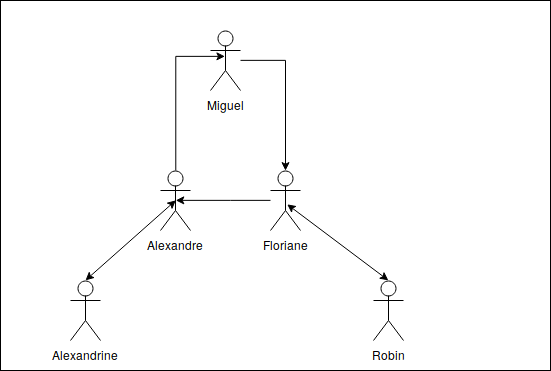
\includegraphics[width=\linewidth]{tp06.png}
\section{Saison 2}
\emph{
Prouvez lui à l’aide des séquents qu’il a forcément tort:
\textbf{soit il y a une relation incestueuse, soit Miguel n’est pas amoureux de Floriane.}}

\subsection*{Transformation en formule du premier ordre:}
\begin{alltt}
  \exists a,b,x,y, Inceste(a,b) \bigvee !Amoureux(x,y)
\end{alltt}

\subsection*{Séquent:}
\begin{alltt}
  \frac{}{\frac{Amoureux(x,y) \vdash Inceste(a,b)}{\frac{\vdash Inceste(a,b) \neg Amoureux(x,y)}{\frac{\vdashInceste(a,b) \bigvee \neg Amoureux(x,y)}{\vdash \exists a,b,x,y, Inceste(a,b) \bigvee \neg Amoureux(x,y)}}}}
\end{alltt}
\end{document}
